\documentclass[twocolumn,preprintnumbers,superscriptaddress]{revtex4-2}
\usepackage{amsmath}
\usepackage{amssymb}
\usepackage{graphicx}
\usepackage{hyperref}
\usepackage{physics}
\usepackage{xcolor}
\usepackage{xspace,slashed}
\usepackage{qcircuit}
\usepackage{multirow}
\usepackage[utf8]{inputenc}
\usepackage{subfigure}

\usepackage{array}

\begin{document}

\title{
  Style-based Quantum Generative Adversarial Networks for Monte Carlo events
}

\preprint{CERN-TH-xx, TIF-UNIMI-2021-xx}

\newcommand{\CERNaff}{Theoretical Physics Department, CERN, CH-1211
  Geneva 23, Switzerland.}

\newcommand{\tii}{Quantum Research Centre, Technology Innovation Institute, Abu Dhabi, UAE}

\newcommand{\bern}{Albert Einstein Center, CH-3012 Bern, Switzerland}

\newcommand{\UB}{Departament de F\'isica Qu\`antica i Astrof\'isica and Institut de Ci\`encies del Cosmos (ICCUB), Universitat de Barcelona, Barcelona, Spain.}

\newcommand{\MIaff}{TIF Lab, Dipartimento di Fisica, Universit\`a degli Studi di
  Milano and INFN Sezione di Milano, Milan, Italy.}

\author{Carlos Bravo-Prieto}
\affiliation{\tii}
\affiliation{\UB}

\author{Julien Baglio}
\affiliation{\CERNaff}

\author{Marco C\`e}
\affiliation{\CERNaff}

\author{Anthony Francis}
\affiliation{\bern}

\author{Dorota Grabowska}
\affiliation{\CERNaff}

\author{Stefano Carrazza}
\affiliation{\MIaff}
\affiliation{\CERNaff}
\affiliation{\tii}


\begin{abstract}
  We present a first attempt to design a quantum circuit for the generation of
  Monte Carlo simulated events using quantum generative models, in the context
  of high energy physics (HEP). The growing interest in quantum computing and
  the recent developments of new algorithms and quantum hardware devices
  motivates the study of methodologies applied to HEP. In this work we
  identify architectures of variational quantum circuits suitable for
  designing a generative model for Monte Carlo event generation. We validate
  the methodology by performing experiments on artificial data generated from
  known underlying distributions. Finally, we model Monte Carlo simulated
  events and benchmark the performance in terms of quality and performance.
\end{abstract}

\maketitle

\section{Introduction}

Quantum computing is a new paradigm whereby quantum phenomena are harnessed to
perform computations. The current availability of noisy intermediate-scale
quantum computers (NISQ)~\cite{nisq}, and recent achievements such as quantum
computational supremacy~\cite{supremacy, zhong2020quantum}, have led to a
growing interest in these devices to perform computational tasks faster than any
classical machine. Among many of the near-term
applications~\cite{cerezo2021variational, bharti2021noisy}, the field of Quantum
Machine Learning (QML)~\cite{biamonte2017quantum, schuld2018supervised} is held
as one of the most promising approaches to make use of NISQ computers.

Early work in QML was mostly focused on speeding up linear algebra
subroutines~\cite{wiebe2012quantum, lloyd:2013ml, Rebentrost:2014svm,
  kerenidis2020quantum}, widely used in classical machine learning, by leveraging
the HHL algorithm~\cite{harrow2009quantum}. Notice that this approach holds
promise for the future, when large-scale quantum computers exist with low gate
errors and enough qubits to perform quantum error correction. On the other hand, more
recent proposals suggest using the quantum devices to define a quantum neural network (QNN), or parameterized
quantum circuit~\cite{benedetti2019parameterized, sim2019expressibility,
  bravo2020scaling}, which then can be trained to
implement a function class~\cite{schuld2021effect, goto2021universal,
  perez2021one}. For example, several QNNs have been proposed for pattern
classification~\cite{havlivcek2019supervised, Schuld:2020circuit,
  perezsalinas:2020reuploading} or data compression~\cite{romero2017quantum,
  bravo2021quantum, cao2021noise}. Interestingly, this QML approach to quantum
computing is a research topic that can be adapted, improved, and tested on many
research problems. Motivated by this idea, we propose to investigate the
possibility to use QNNs for generative modeling~\cite{benedetti2019generative,
  hamilton2019generative, coyle2020born}. More specifically, for the generation of
Monte Carlo events through quantum generative adversarial networks
(qGANs)~\cite{dallaire2018quantum, lloyd2018quantum}.

The generative adversarial framework employs two competing networks that are
trained alternatively, the generator and the
discriminator~\cite{goodfellow2014generative}. The generator produces candidates
while the discriminator evaluates them. The objective of the discriminator is to
distinguish the real samples from the generated ones. That is, the discriminator
plays the role of the generator's adversary, and therefore, their competition is
a zero-sum two-player game. Substituting either the discriminator, the
generator, or both with quantum systems we translate the scheme to quantum
computing.

In recent months, the spreading interest in QML has led to different qGAN
implementations~\cite{zoufal2019quantum, zeng2019learning, situ2020quantum,
  hu2019quantum, benedetti2019adversarial, romero2021variational,
  niu2021entangling}. However, our contribution here can be summarized in three
distinct aspects. (1) Previous proposals employ toy data for their qGAN
training. Moreover, in some cases, it is classical data. It has been recently
conjectured that if QML ever provides any speed up, it will likely appear from
learning the data of a quantum process~\cite{huang2021information,
  kubler2021inductive}. Therefore, we first train and validate our qGAN model with
artificial data from known underlying probability density functions. Then, in
order to test our model in a realistic setup, we use as training set simulated
Monte Carlo events for particle physics processes at the Large Hadron Collider
(LHC) at CERN. (2) We propose an alternative quantum generator architecture. In contrast to
previous proposals where the prior noise distribution, or latent dimension, is
encoded at the beginning of the generator, we instead encode it on every layer
of the network. This permits to the new generator to process and decide in which
parts of the network the latent variables should play a relevant role. This
allowed us to achieve improved state-of-the-art results with shallow QNNs using
adversarial learning. Let us remark as well that this has been proven extremely
useful in the classical context~\cite{karras2019style}. (3) We validate and
assess our qGAN in quantum hardware. Specifically, we successfully implement our
model in two different quantum architectures, namely, ion traps and
superconducting qubits.

It is important to highlight that several research groups from the high-energy
physics (HEP) community are investigating potential applications of quantum
technologies in HEP applications and obtaining interesting
results~\cite{P_rez_Salinas_2021,Guan_2021,chang2021quantum,Chang_2021,Belis_2021,khattak2021fast}.
Therefore, the study presented in this manuscript should be considered as
proof-of-concept, providing a robust and reproducible starting point for future
investigations. In particular, the introduction of GAN models in HEP Monte Carlo
simulation has been discussed extensively in the last years, see
Ref.~\cite{baldi2021gan,Backes_2021,butter2020generative,Butter_2021,Butter_2020,Bellagente_2020,Butter_2019}.
In this work we consider the possibility to use a qGAN model in a data
augmentation context, where the model is trained with a small amount of input
samples and it learns how to sample the underlying distribution with reliable
results.

% To be modified
The paper is structured as follows. In Sec.~\ref{sec:implementation} we identify
the best qGAN architecture for sampling. In Sec.~\ref{sec:validation} we
validate the qGAN model using toy data. Then, in Sec.~\ref{sec:lhc} we train the qGAN
generator on simulated LHC events. Finally, in Sec.~\ref{sec:deployment} we test
our final model on real quantum hardware and in Sec.~\ref{sec:conclusion} we
present our conclusion and future development directions.

\section{Implementation}
\label{sec:implementation}

\subsection{Workflow design}

The classical implementation of a GAN model~\cite{goodfellow2014generative}
involves at least three required components: the discriminator model, the
generator model, and the adversarial training procedure. In this work, we
consider a hybrid quantum-classical system, where the generator model has a
quantum representation through a QNN, while the
discriminator is a classical neural network model. This choice is motivated by
the practical positive implications of a hardware based generative model, in
particular, the possibility to obtain performance improvements in a real quantum
device. In fact, the idea of using a quantum device for the generation of
samples, by delegating the complicated aspects of density modeling and sampling
to a hardware architecture, is very attractive.
%
There are alternative approaches where both models could be represented by a
QNN~\cite{add_cite}, however after testing some prototype architectures we
have observed faster convergence when using a classical discriminator.

In Figure~\ref{fig:scheme} we show schematically the steps involved in the qGAN
presented here. The procedure starts from the preparation of samples from a
known distribution function that we would like to encode in the quantum
generator model. At the same time, we define a QNN model where
we inject stochastic noise in the latent space variables which are used to
define quantum gates. The generator model is then used to extract fake samples
that after the training procedure should match the quality of the known input
distribution. Both sets of samples are then used to train the discriminator
model. The quality of the training is measured by an appropriate loss function
which is monitored and optimized classically by a minimization algorithm based on
the adversarial approach. The training process consists of a simultaneous
stochastic gradient descent for both models which after reaching convergence
delivers a quantum generator model with realistic sampling.

In the next paragraphs, we first introduce the Ansatz model for the quantum
generator network and validate the procedure by using samples from known
distribution functions and quantum simulation on classical hardware. Then, we
train our qGAN model with Monte Carlo generated LHC events using quantum
simulation. Finally, the best-trained model is deployed on real quantum hardware
devices based on superconducting and trapped ion technologies.

All calculations involving quantum circuits simulation are performed using the
{\tt Qibo} v0.1.6~\cite{efthymiou2020qibo,stavros_efthymiou_2021_5088103} on
classical hardware. For this particular project, we have used the {\tt
tensorflow}~\cite{tensorflow2015-whitepaper} backend which provides the
possibility to use gradient descent optimizers during the training step. The
qGAN model is publicly available through the {\tt Qibo} API. The experimental
implementation of this model was done using {\tt
Qiskit}~\cite{gadi_aleksandrowicz_2019_2562111} from the {\tt
OpenQASM}~\cite{cross2017open} code generated by {\tt Qibo}.

{\color{red}[SC: Marco, Julien please include other packages you have used for IonQ/IBM.]}

\begin{figure}
  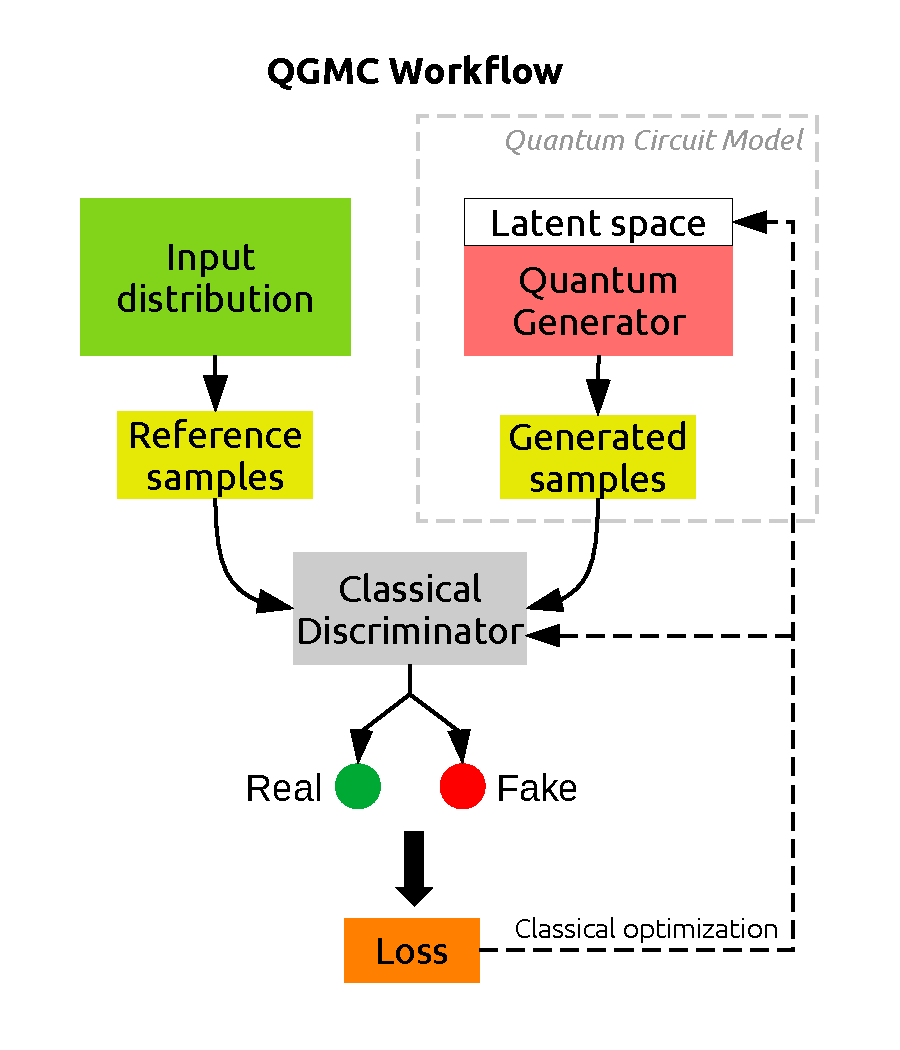
\includegraphics[width=0.4\textwidth]{plots/scheme.pdf}
  \caption{\label{fig:scheme} Schematic steps involved in the qGAN training.}
\end{figure}

\subsection{Ansatz determination}

{\color{red}[SC: Carlos please describe the model and how the model has been
    obtained.]}

\begin{itemize}
  \item explain the ansatz structure
  \item describe Figure~\ref{fig:circuit}
  \item include technical details concerning the optimization procedure.
\end{itemize}

\begin{figure}
  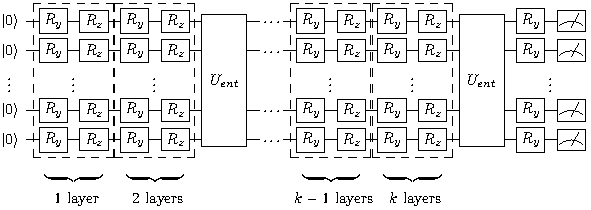
\includegraphics[width=1.0\columnwidth]{plots/ansatz1.pdf}
  \caption{\label{fig:circuit}Ansatz structure for the quantum generator circuit model.}
\end{figure}

\section{Validation examples}
\label{sec:validation}

In this section we show examples of qGAN models obtained for known prior
distribution functions in one and three dimensions. The results presented here
have been obtained after a systematic process of fine tuning and manual
hyper-optimization of the Ansatz model.

\subsection{1D Gamma distribution}

In order to test the framework proposed in the paragraph above, we have
considered the sampling of a 1D gamma distribution with probability density
function reading
\begin{equation}
  p_\gamma (x, \alpha, \beta) = x^{\alpha-1} \frac{e^{-x/\beta}}{\beta^\alpha \Gamma(\alpha)},
\end{equation}
where $\Gamma$ is the Gamma function. In this example we take $p_\gamma (x, 1, 1)$ as input distribution
and train a qGAN with 1 qubit, using $10^4$ samples from the input distribution.
%
In Figure~\ref{fig:loss} we show the evolution of the loss function for the
generator and discriminator models in terms number of epochs. We observe the
typical behaviour of GAN training and a convergence region after 15000 epochs.
%
The qGAN is trained with batch sizes of 128 samples.

\begin{figure}
  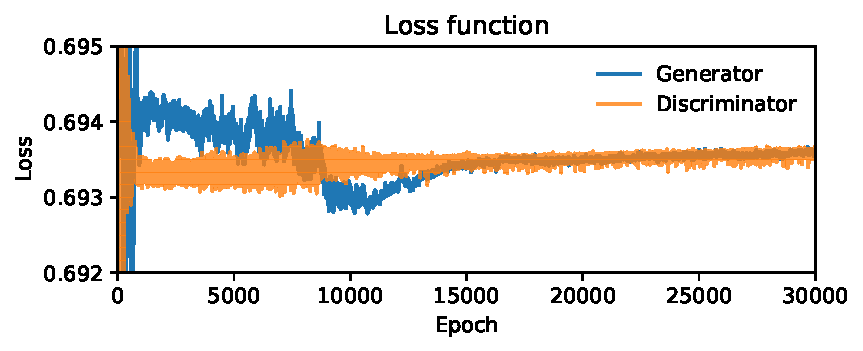
\includegraphics[width=0.5\textwidth]{plots/1Dgamma/1Dgamma_loss.pdf}
  \caption{\label{fig:loss}Example of loss function convergence. After an
  initial warn-up phase the loss function of both models converge.}
\end{figure}

The image on the top of Figure~\ref{fig:gamma} compares the output generated by
the qGAN model (blue histogram) with the reference input distribution function
(red histogram) for $10^4$ samples. We observe that the distributions are
statistically similar, in fact, the Kullback-Leibler divergence
(KL)~\cite{kullback1951information} between both distributions is 0.141.
%
In order to verify the quality of the qGAN model, we compare both distribution
with $10^5$ samples in the bottom image of Figure~\ref{fig:gamma}. In this case,
the number of sampled points is one order of magnitude larger than input
training set. The agreement between both distribution is remarkably good,
obtaining a small KL distance of 0.041
%
This behaviour confirms that the qGAN model is able to learn the underlying
distribution function even if trained with a small training sample set. Such
feature is particularly interesting in a context of data augmentation
applications~\cite{frid2018synthetic,tanaka2019data}, where few samples are available the qGAN model can
generalize and learn the underlying distribution with satisfactory outcome.

\begin{figure}
  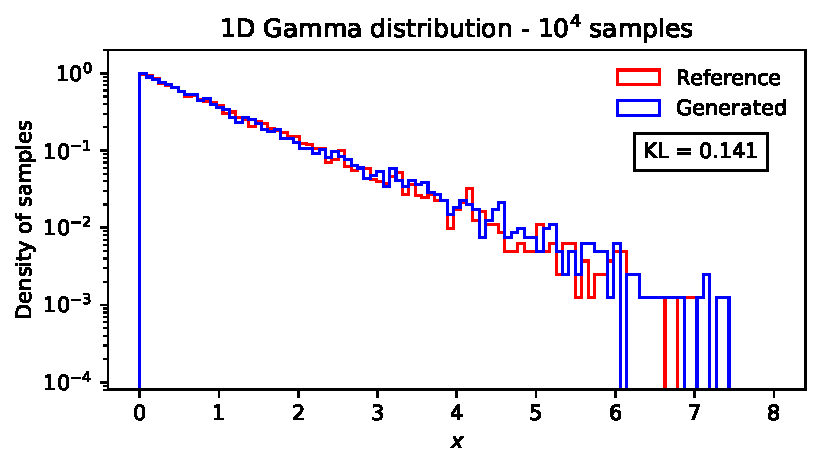
\includegraphics[width=0.45\textwidth]{plots/1Dgamma/1Dgamma_distribution_10k.pdf}
  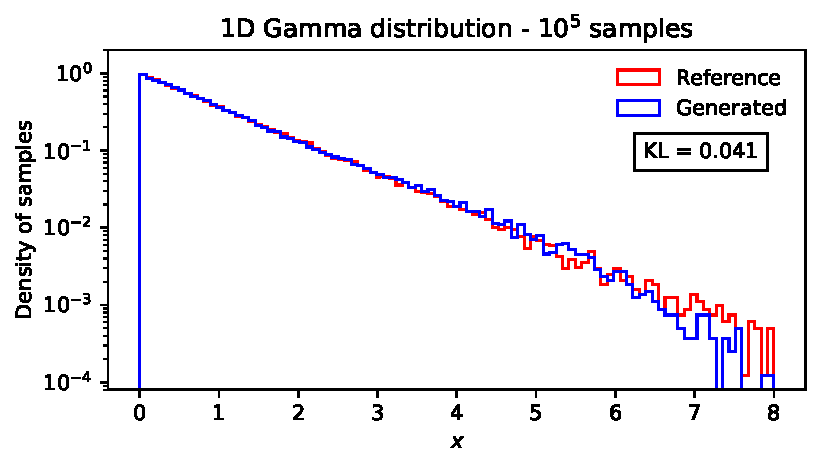
\includegraphics[width=0.45\textwidth]{plots/1Dgamma/1Dgamma_distribution_100k.pdf}
  \caption{\label{fig:gamma} Examples of 1D gamma distribution sampling for the
  reference underlying distribution (red) and the qGAN model (blue) trained with
  $10^4$ samples. On the top we compare the $10^4$ samples, while the figure in
  the bottom shows $10^5$ samples. We observe a good level of agreement between
  both distributions with low values of the Kullback-Leibler distance.}
\end{figure}

\subsection{3D Gaussian distribution}


% \begin{figure*}
%   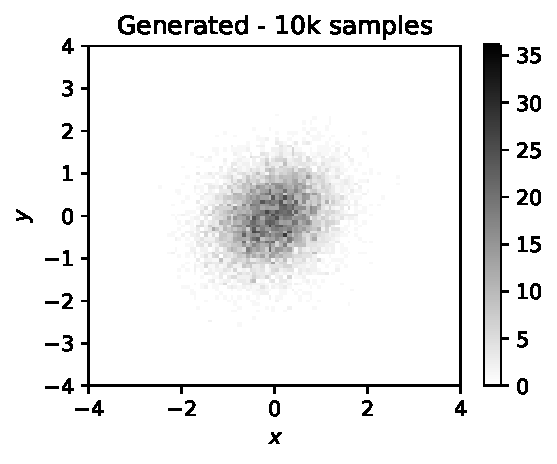
\includegraphics[width=0.3\textwidth]{plots/3Dgaussian_posdef/1-2_FAKE_10k.pdf}%
%   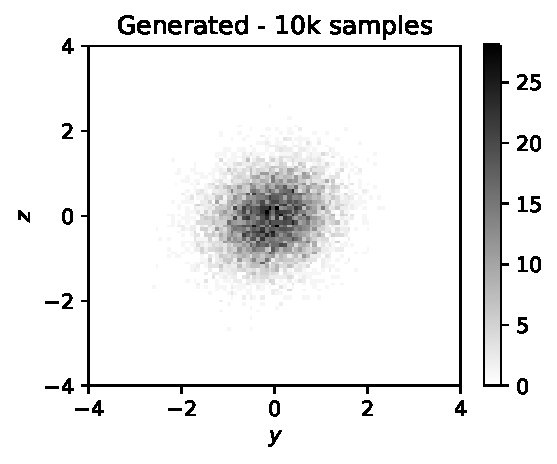
\includegraphics[width=0.3\textwidth]{plots/3Dgaussian_posdef/2-3_FAKE_10k.pdf}%
%   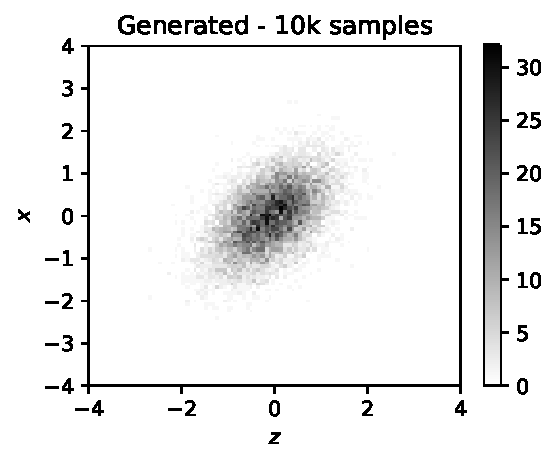
\includegraphics[width=0.3\textwidth]{plots/3Dgaussian_posdef/3-1_FAKE_10k.pdf}

%   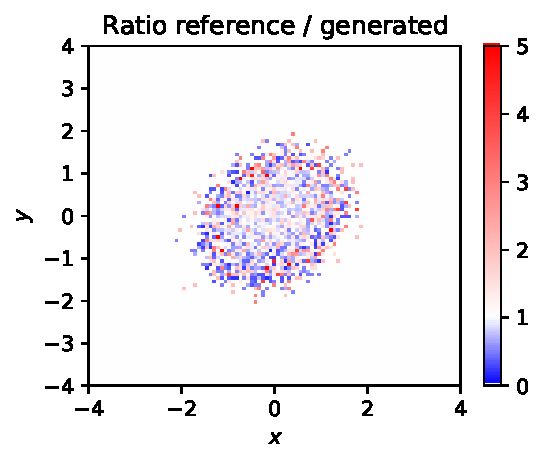
\includegraphics[width=0.3\textwidth]{plots/3Dgaussian_posdef/1-2_RATIO_10k.pdf}%
%   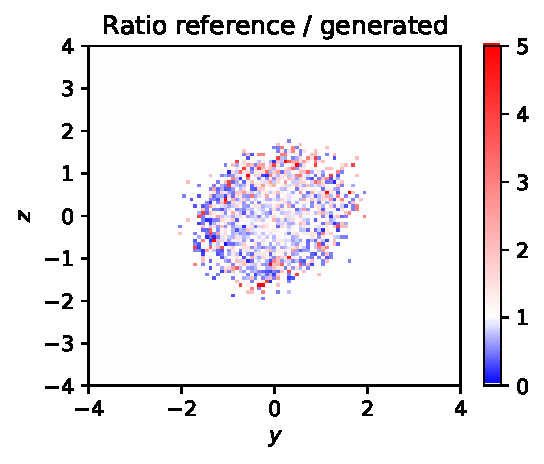
\includegraphics[width=0.3\textwidth]{plots/3Dgaussian_posdef/2-3_RATIO_10k.pdf}%
%   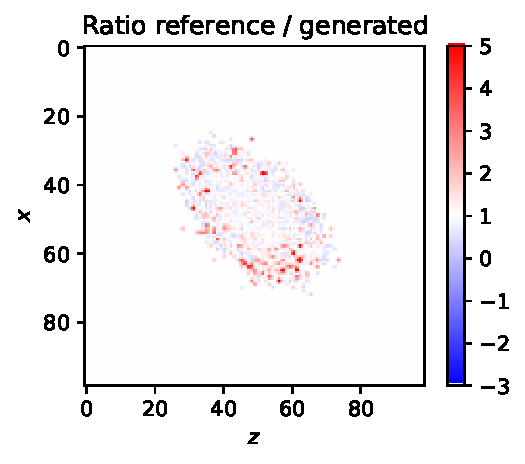
\includegraphics[width=0.3\textwidth]{plots/3Dgaussian_posdef/3-1_RATIO_10k.pdf}

%   \caption{\label{fig:3dgauss}Example of samples generated for a 3D correlated
%     multivariate normal distribution using a QGAN generator model 10k samples.}
% \end{figure*}

\begin{figure*}
  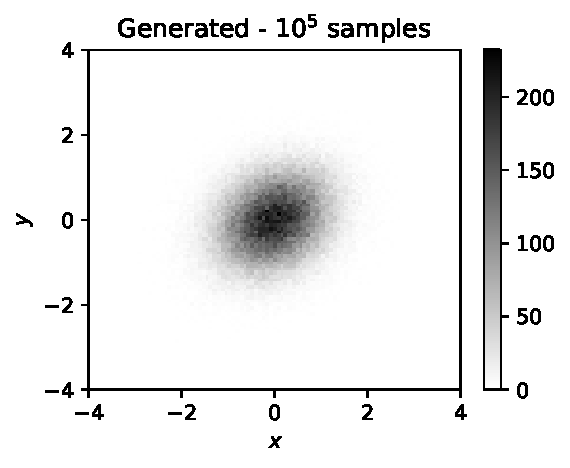
\includegraphics[width=0.3\textwidth]{plots/3Dgaussian_posdef/1-2_FAKE_100k.pdf}%
  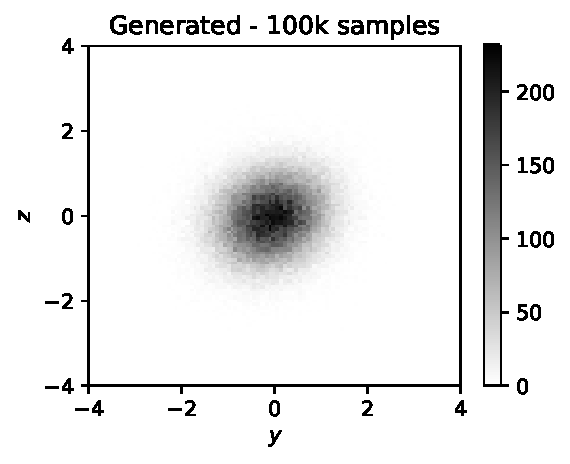
\includegraphics[width=0.3\textwidth]{plots/3Dgaussian_posdef/2-3_FAKE_100k.pdf}%
  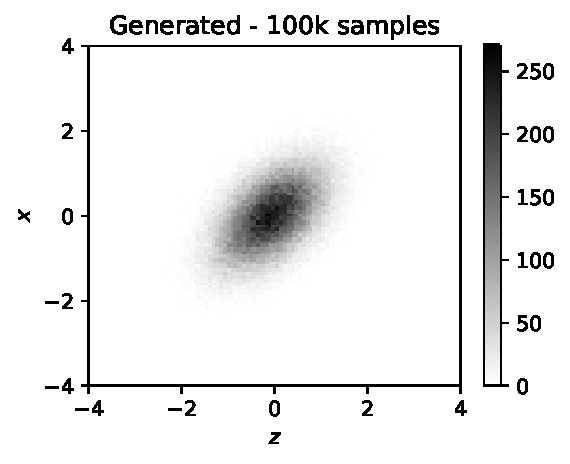
\includegraphics[width=0.3\textwidth]{plots/3Dgaussian_posdef/3-1_FAKE_100k.pdf}

  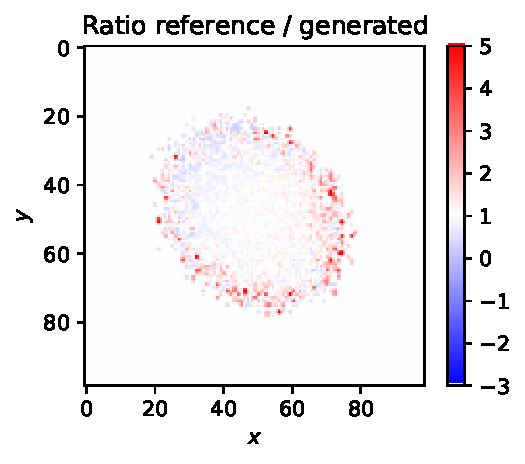
\includegraphics[width=0.3\textwidth]{plots/3Dgaussian_posdef/1-2_RATIO_100k.pdf}%
  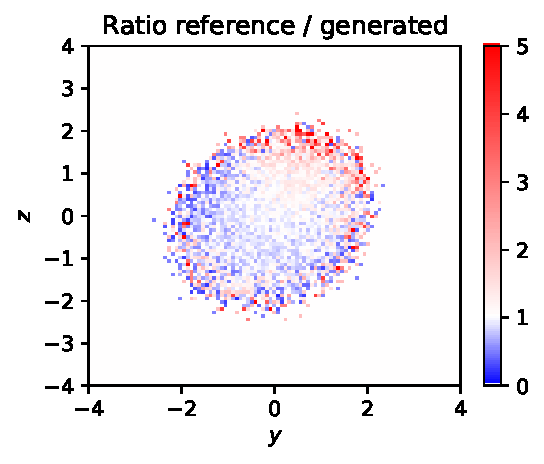
\includegraphics[width=0.3\textwidth]{plots/3Dgaussian_posdef/2-3_RATIO_100k.pdf}%
  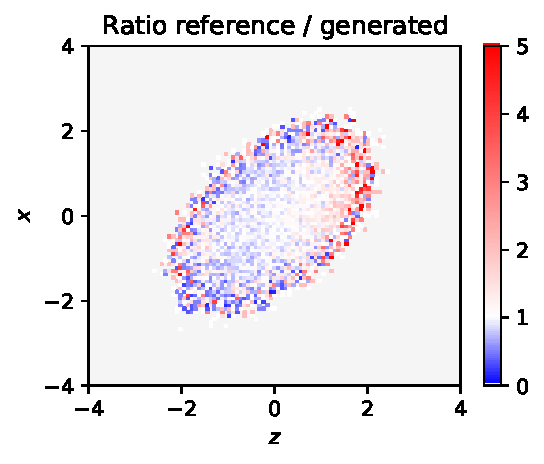
\includegraphics[width=0.3\textwidth]{plots/3Dgaussian_posdef/3-1_RATIO_100k.pdf}

  \caption{\label{fig:3dgauss}Example of samples generated for a 3D correlated
    multivariate normal distribution using a QGAN generator model 100k samples from 10k training set.}
\end{figure*}

\begin{figure*}
  % 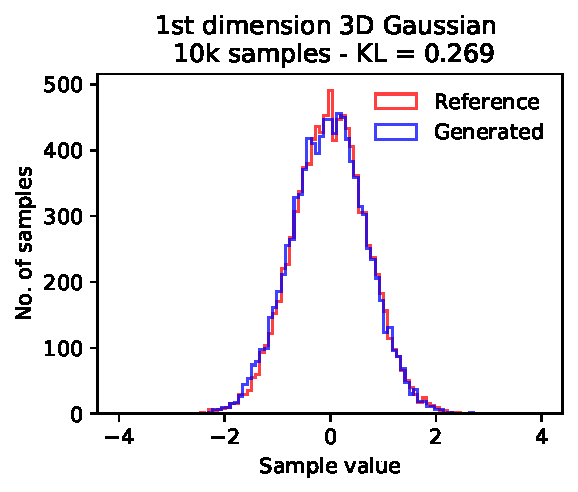
\includegraphics[width=0.3\textwidth]{plots/3Dgaussian_posdef/1-distribution_3dgaussian_10k.pdf}%
  % 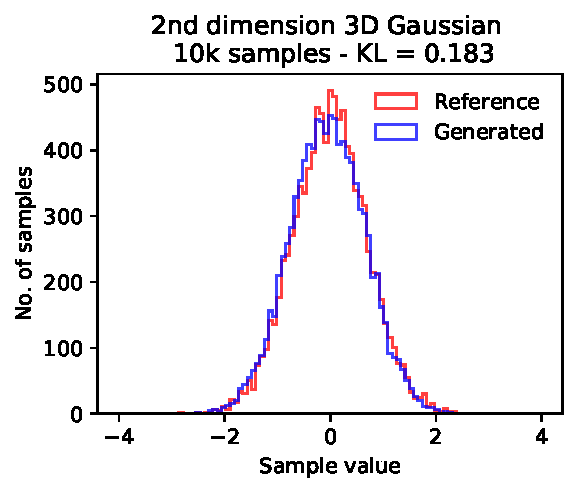
\includegraphics[width=0.3\textwidth]{plots/3Dgaussian_posdef/2-distribution_3dgaussian_10k.pdf}%
  % 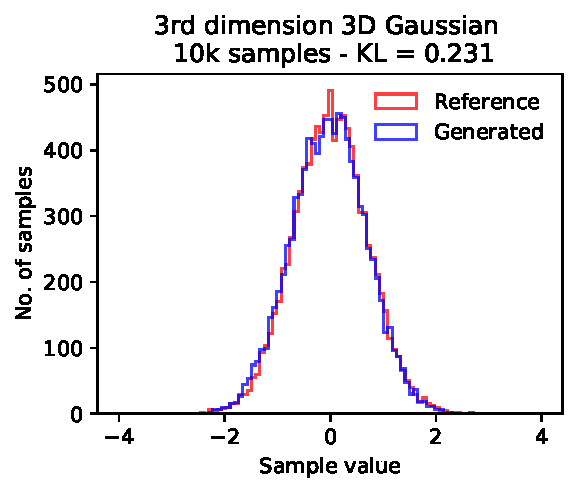
\includegraphics[width=0.3\textwidth]{plots/3Dgaussian_posdef/3-distribution_3dgaussian_10k.pdf}

  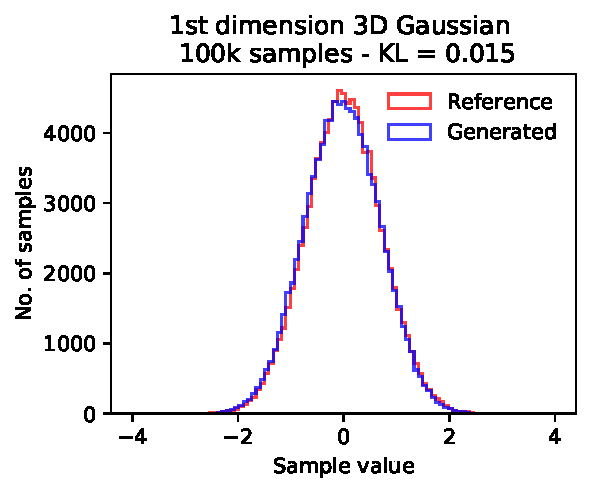
\includegraphics[width=0.3\textwidth]{plots/3Dgaussian_posdef/1-distribution_3dgaussian_100k.pdf}%
  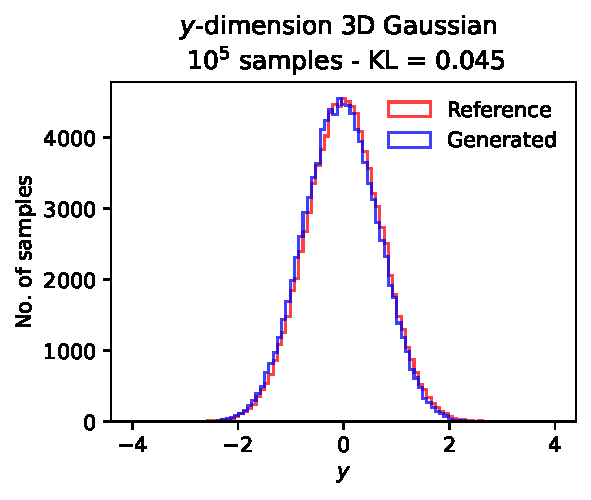
\includegraphics[width=0.3\textwidth]{plots/3Dgaussian_posdef/2-distribution_3dgaussian_100k.pdf}%
  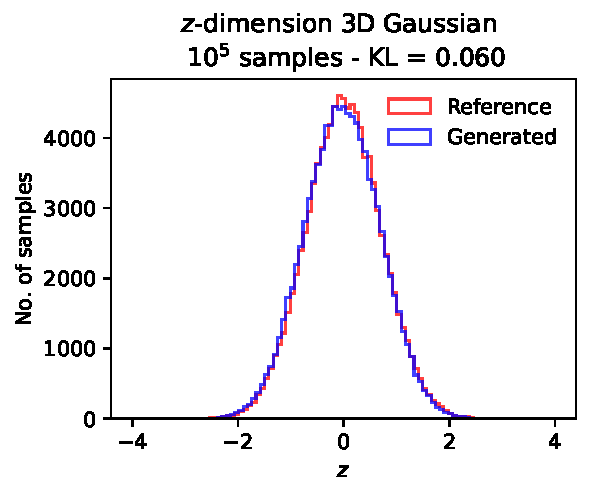
\includegraphics[width=0.3\textwidth]{plots/3Dgaussian_posdef/3-distribution_3dgaussian_100k.pdf}

  \caption{\label{fig:3dgauss}Example of samples generated for a 3D correlated
    multivariate normal distribution using a QGAN generator model.}
\end{figure*}

\begin{table}
  \begin{tabular}{l|c|c}
     & {\bf 1D gamma} & {\bf 3D gaussian} \tabularnewline
    \hline
    Qubits & 1 & 3 \tabularnewline
    Latent dim & 1 & 3 \tabularnewline
    Layers & 1 & 1 \tabularnewline
    Epochs & $3\times10^4$ & $1.3\times10^4$ \tabularnewline
    Parameters & 10 & 34 \tabularnewline
    $U_{\rm ent}$ & None & 2 sequential C$R_y$ gates \tabularnewline
    \hline
  \end{tabular}

  \caption{\label{table:summary} Summary of the Ansatz parameters for the 1D
  gamma distribution and the 3D gaussian distribution.}

\end{table}

Finally, in Table~\ref{table:summary} we summarize the qGAN configurations
obtained for both examples.

\section{Generating LHC events}
\label{sec:lhc}

\begin{enumerate}
  \item Show ttbar and WW results, histograms, KL, correlations, etc.
  \item Provide hints concerning data augmentation.
  \item Show experimental results obtained with quantum hardware, identify the
        best features, pro and cons of different hardware.
\end{enumerate}

% \begin{figure*}
%   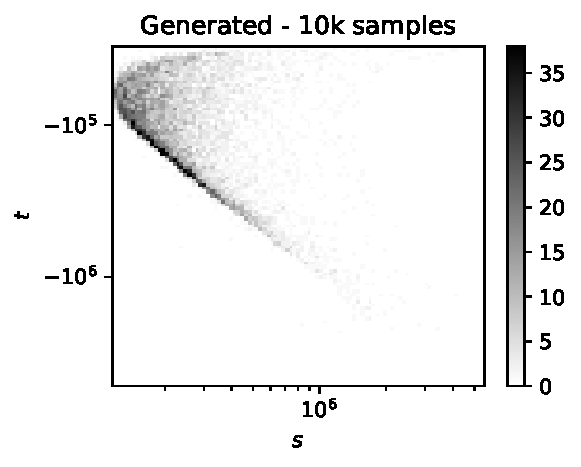
\includegraphics[width=0.32\textwidth]{plots/LHCttbar/s-t_FAKE_10k.pdf}%
%   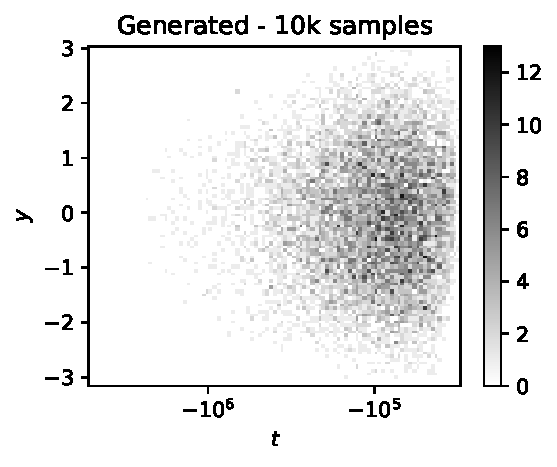
\includegraphics[width=0.305\textwidth]{plots/LHCttbar/t-y_FAKE_10k.pdf}%
%   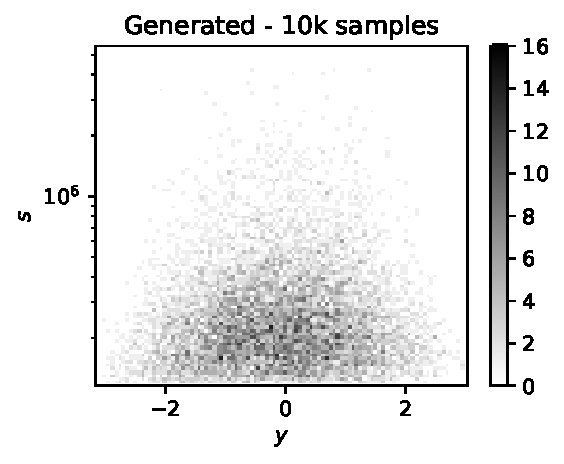
\includegraphics[width=0.31\textwidth]{plots/LHCttbar/y-s_FAKE_10k.pdf}

%   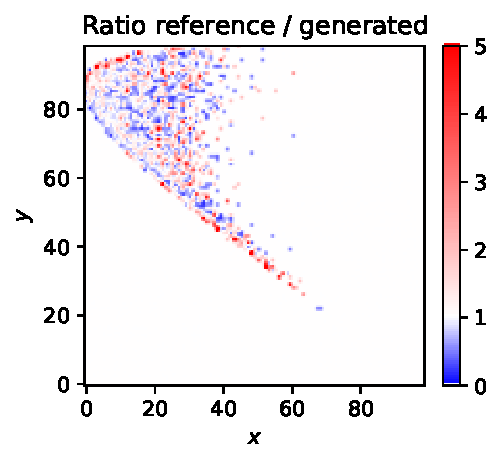
\includegraphics[width=0.32\textwidth]{plots/LHCttbar/s-t_RATIO_10k.pdf}%
%   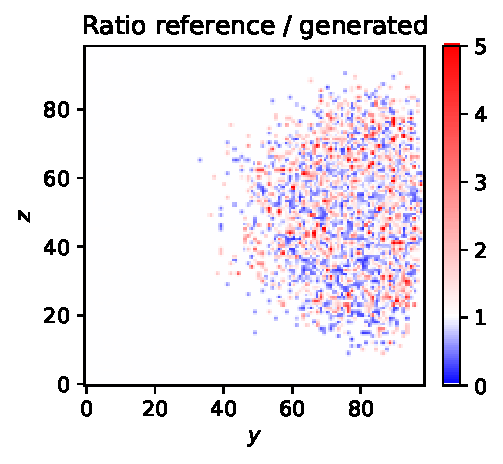
\includegraphics[width=0.305\textwidth]{plots/LHCttbar/t-y_RATIO_10k.pdf}%
%   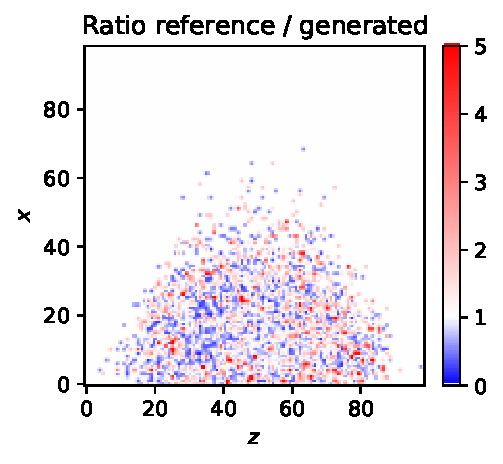
\includegraphics[width=0.31\textwidth]{plots/LHCttbar/y-s_RATIO_10k.pdf}

%   \caption{\label{fig:3dgauss}Example of samples generated for a $t\bar{t}$
%     production using a QGAN generator model.}
% \end{figure*}

\begin{figure*}
  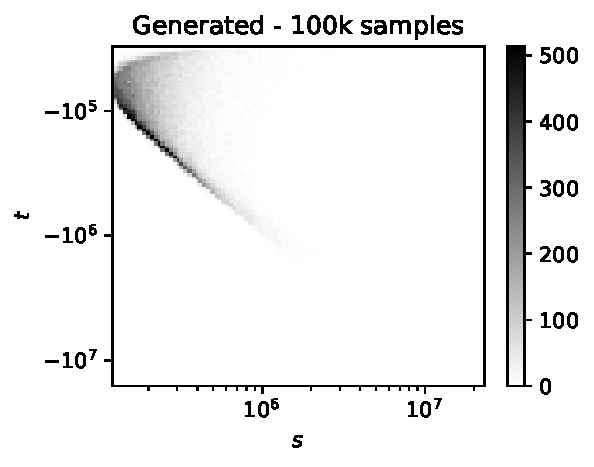
\includegraphics[width=0.32\textwidth]{plots/LHCttbar/s-t_FAKE_100k.pdf}%
  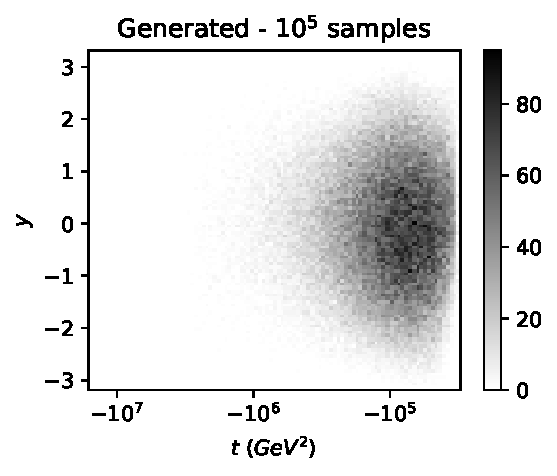
\includegraphics[width=0.3\textwidth]{plots/LHCttbar/t-y_FAKE_100k.pdf}%
  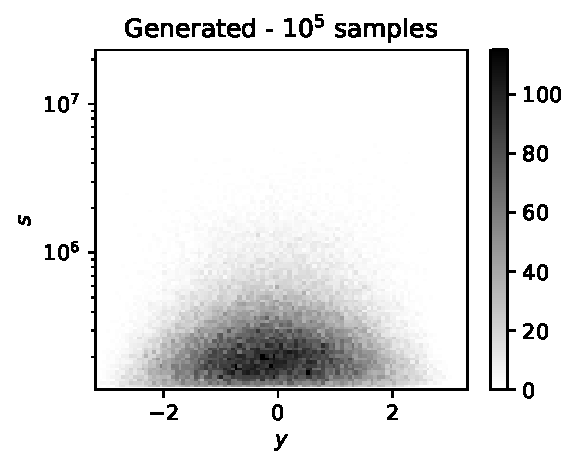
\includegraphics[width=0.31\textwidth]{plots/LHCttbar/y-s_FAKE_100k.pdf}

  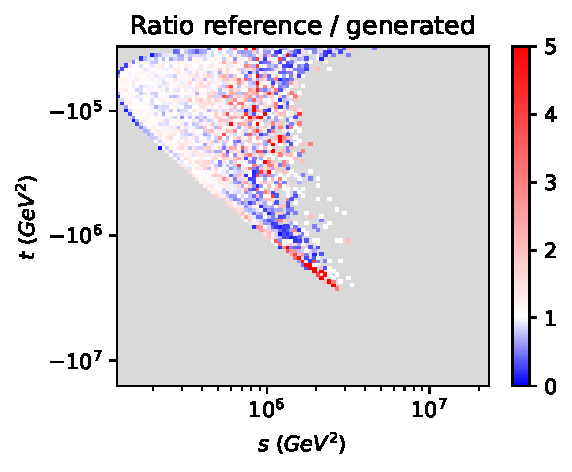
\includegraphics[width=0.32\textwidth]{plots/LHCttbar/s-t_RATIO_100k.pdf}%
  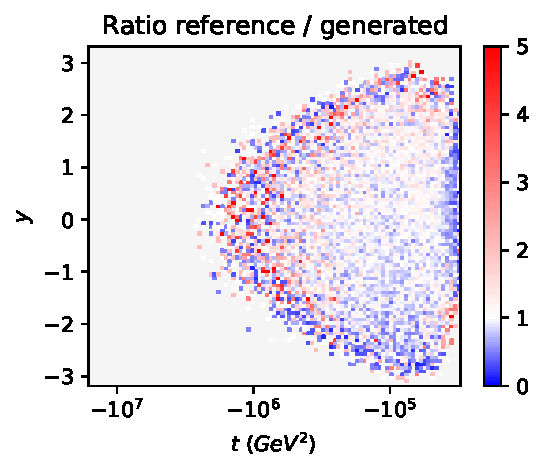
\includegraphics[width=0.3\textwidth]{plots/LHCttbar/t-y_RATIO_100k.pdf}%
  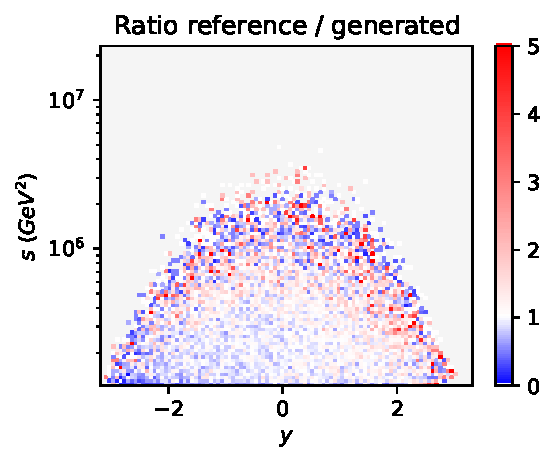
\includegraphics[width=0.31\textwidth]{plots/LHCttbar/y-s_RATIO_100k.pdf}

  \caption{\label{fig:3dgauss}Example of samples generated for a $t\bar{t}$
    production using a QGAN generator model.}
\end{figure*}

\begin{figure*}

  % 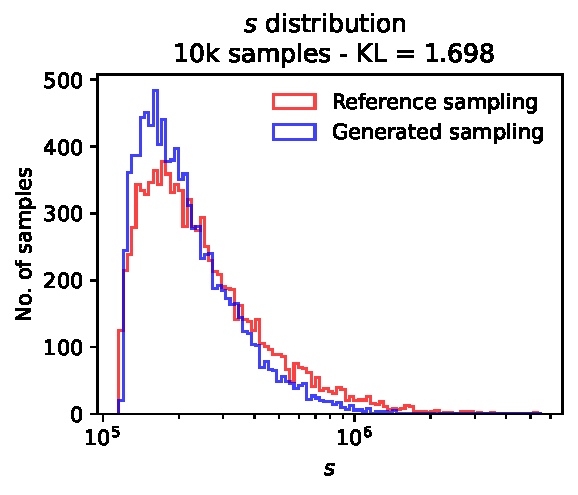
\includegraphics[width=0.3\textwidth]{plots/LHCttbar/s-distribution_LHCdata_10k.pdf}%
  % 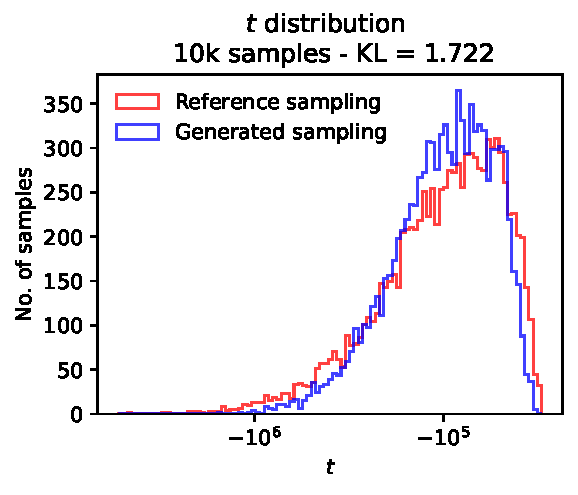
\includegraphics[width=0.3\textwidth]{plots/LHCttbar/t-distribution_LHCdata_10k.pdf}%
  % 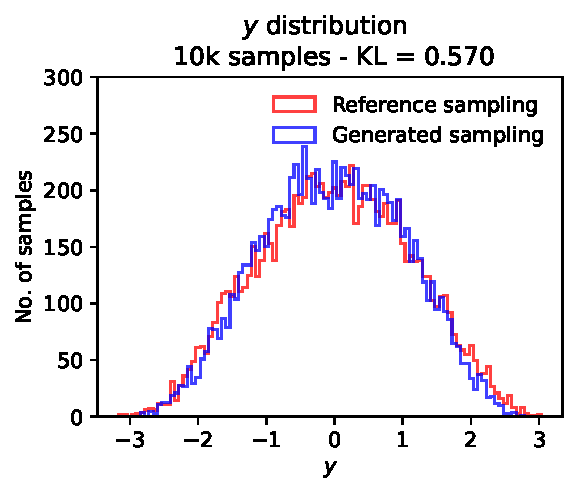
\includegraphics[width=0.3\textwidth]{plots/LHCttbar/y-distribution_LHCdata_10k.pdf}

  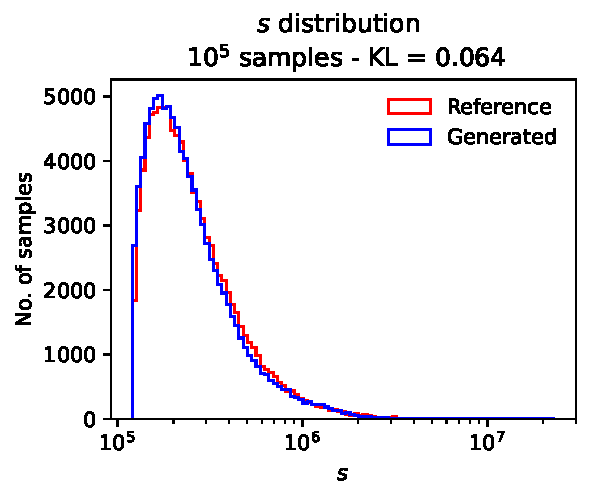
\includegraphics[width=0.3\textwidth]{plots/LHCttbar/s-distribution_LHCdata_100k.pdf}%
  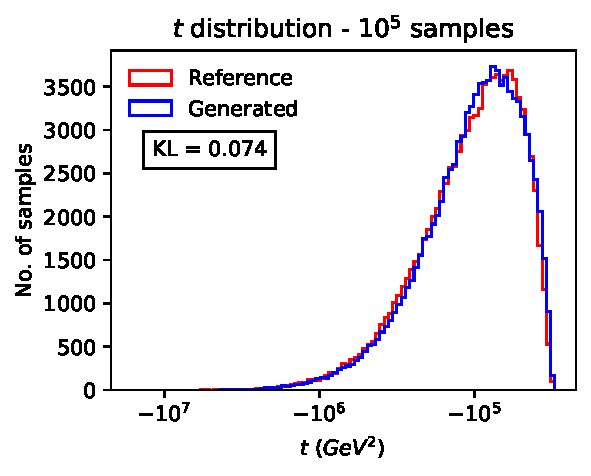
\includegraphics[width=0.3\textwidth]{plots/LHCttbar/t-distribution_LHCdata_100k.pdf}%
  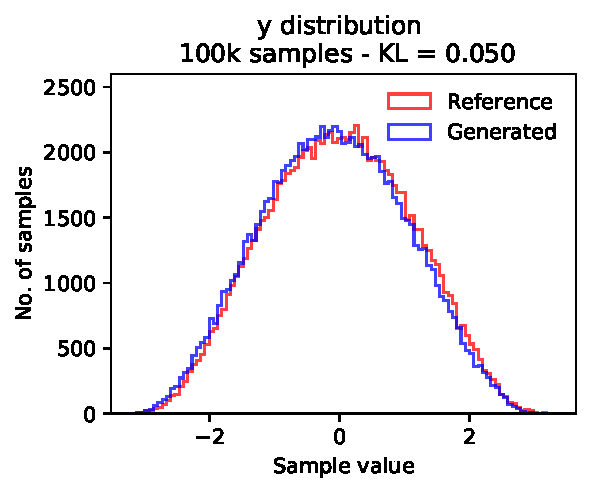
\includegraphics[width=0.3\textwidth]{plots/LHCttbar/y-distribution_LHCdata_100k.pdf}

  \caption{\label{fig:3dgauss}Example of samples generated for a $t\bar{t}$
    production using a QGAN generator model.}
\end{figure*}

\section{Sampling from real quantum hardware}
\label{sec:deployment}

{\color{red}[SC: Julien and Marco please summarize the experimental setup]}

\begin{figure*}

  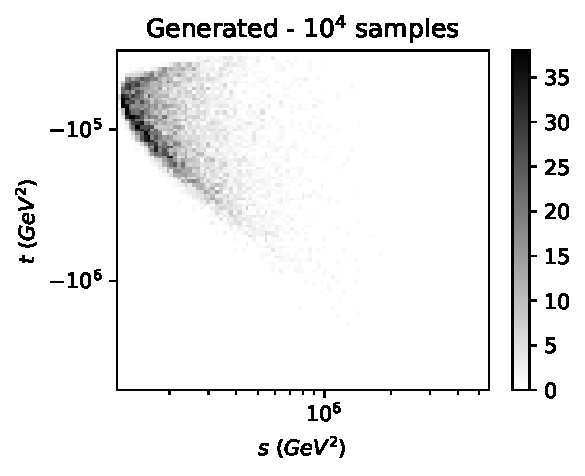
\includegraphics[width=0.32\textwidth]{plots/hardware_1k/ibm_lagos/s-t_FAKE_IBM_10k.pdf}%
  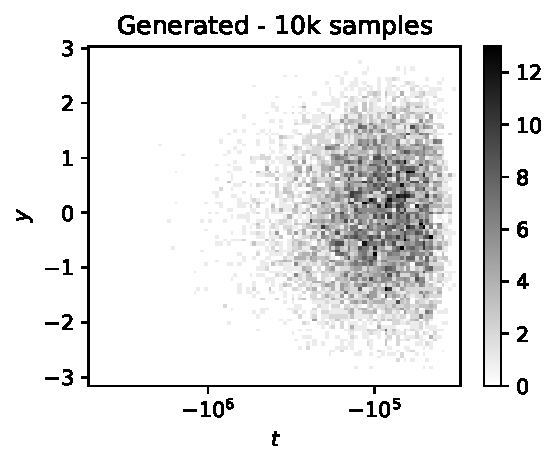
\includegraphics[width=0.305\textwidth]{plots/hardware_1k/ibm_lagos/t-y_FAKE_IBM_10k.pdf}%
  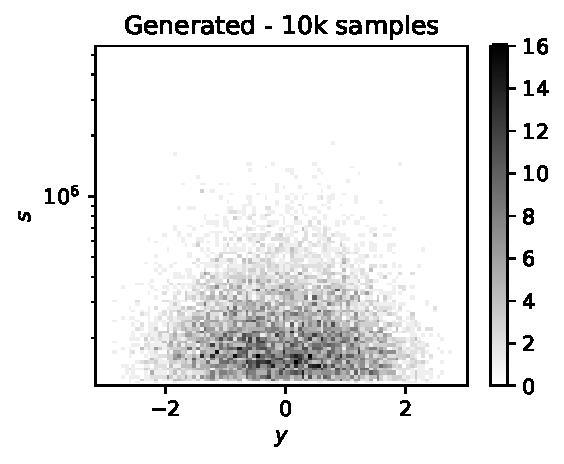
\includegraphics[width=0.31\textwidth]{plots/hardware_1k/ibm_lagos/y-s_FAKE_IBM_10k.pdf}

  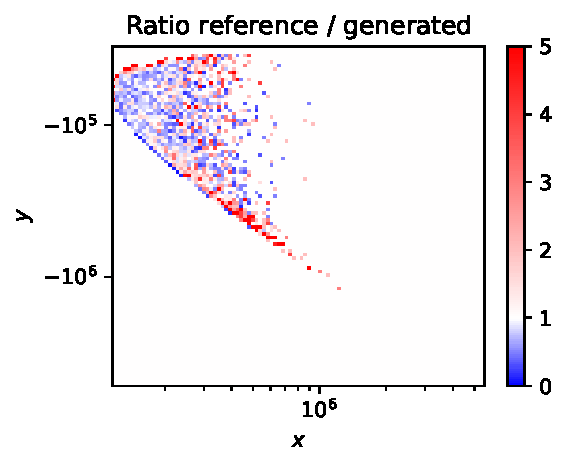
\includegraphics[width=0.32\textwidth]{plots/hardware_1k/ibm_lagos/s-t_RATIO_IBM_10k.pdf}%
  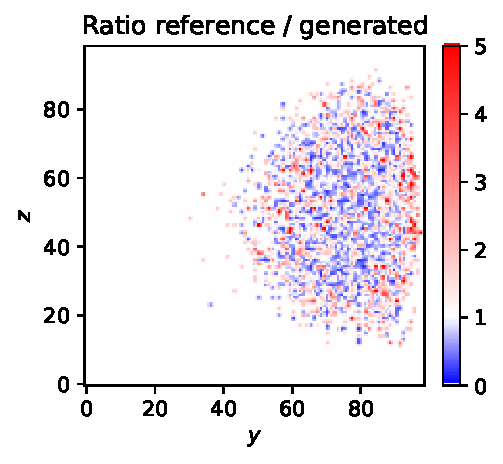
\includegraphics[width=0.305\textwidth]{plots/hardware_1k/ibm_lagos/t-y_RATIO_IBM_10k.pdf}%
  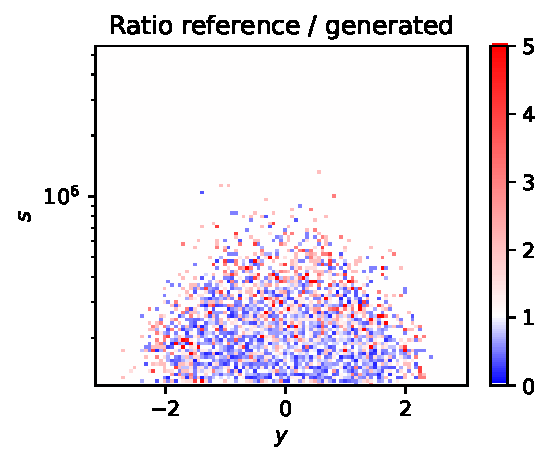
\includegraphics[width=0.31\textwidth]{plots/hardware_1k/ibm_lagos/y-s_RATIO_IBM_10k.pdf}

  \caption{\label{fig:3dgauss}Example of samples generated for a $t\bar{t}$
    production using a QGAN generator model on IBM Lagos.}
\end{figure*}

\begin{figure*}
  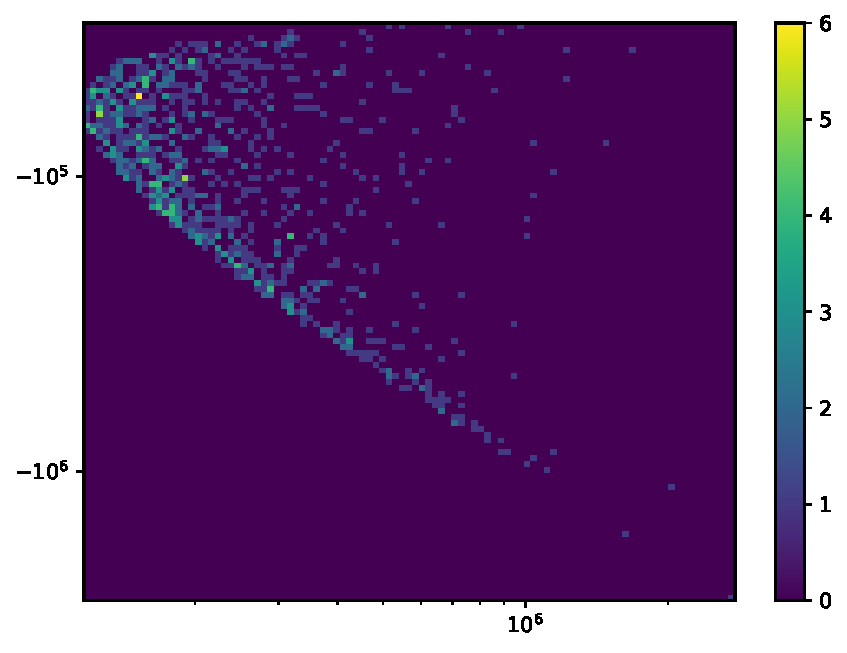
\includegraphics[width=0.25\textwidth]{plots/hardware_1k/ionQ/s-t_REAL_1000_100.pdf}%
  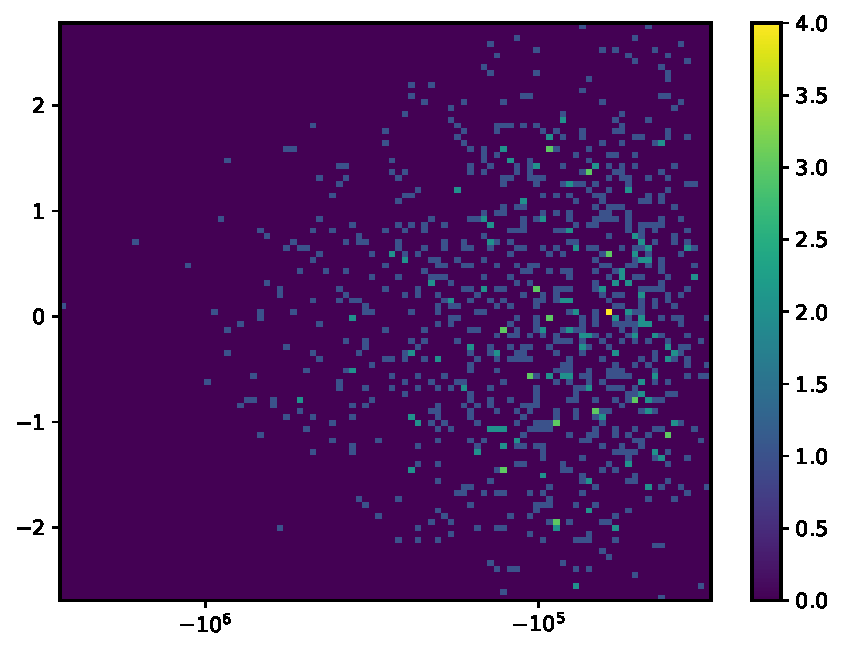
\includegraphics[width=0.25\textwidth]{plots/hardware_1k/ionQ/t-y_REAL_1000_100.pdf}%
  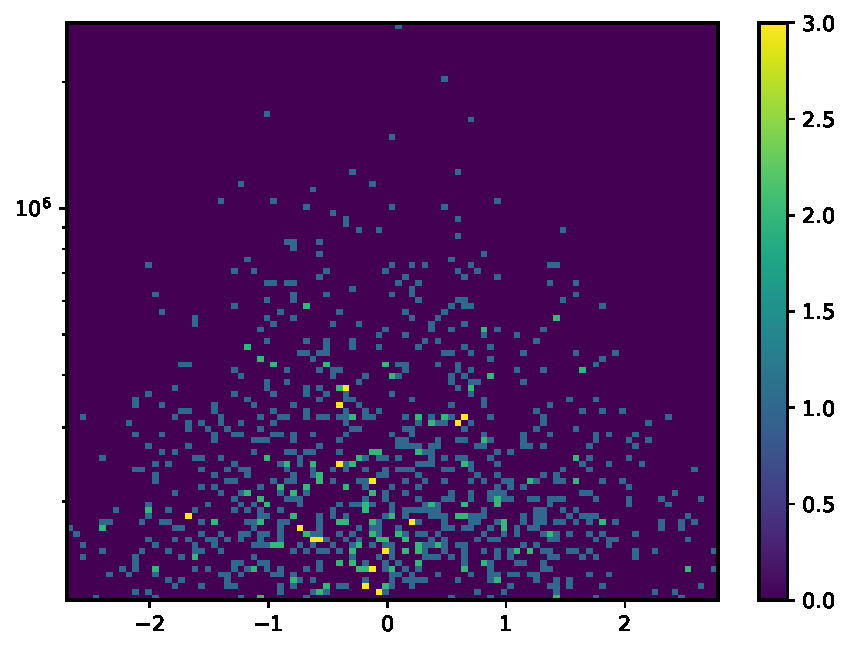
\includegraphics[width=0.25\textwidth]{plots/hardware_1k/ionQ/y-s_REAL_1000_100.pdf}

  \includegraphics[width=0.25\textwidth]{plots/hardware_1k/ionQ/s-t_FAKE_1000_100_3_5_2_10000_128_0.5_1024.pdf}%
  \includegraphics[width=0.25\textwidth]{plots/hardware_1k/ionQ/t-y_FAKE_1000_100_3_5_2_10000_128_0.5_1024.pdf}%
  \includegraphics[width=0.25\textwidth]{plots/hardware_1k/ionQ/y-s_FAKE_1000_100_3_5_2_10000_128_0.5_1024.pdf}

  \caption{\label{fig:3dgauss}Example of samples generated for a $t\bar{t}$
    production using a QGAN generator model on IonQ.}
\end{figure*}


\section{Correlation analysis}

 {\color{red}[SC: Anthony please summarize your results]}

\section{Conclusion}
\label{sec:conclusion}

In this work we proposed variational quantum circuit models for the generation
of Monte Carlo events in the context of high energy physics (HEP). We have
investigated and identified the most suitable Ansatz for the parametrization of
a quantum generative network. Using quantum circuit simulation on classical
hardware, we show that qGAN generators are suitable for Monte Carlo event
simulation.

We highlight some advantages of the qGAN model when compared to the standard
machine learning methodology. From a hardware implementation point of view, the
possibility to write the specific qGAN circuit in a quantum processor, using
its primitives (gates), will accelerate the evaluations and training performance
of Monte Carlo sampling. We expect that real quantum devices will be more
efficient in terms of energy power than classical hardware based on hardware
accelerators such as graphical process units (GPUs).

Furthermore, we propose a reconstruction method for evaluating the qGAN
model in a real quantum device using measurements. This procedure brings all the
difficulties that are typical of experimental quantum hardware, including noise,
error corrections and decoherence. The implementation of accurate and stable
qGAN in a real quantum device still requires the development of hardware
architecture with lower gate error tolerances in comparison to the current
available machines.

On the other hand, our results should be considered as a proof-of-concept
exercise, given that the quantum simulation performance are still not
competitive with an equivalent machine learning implementation. The qGAN
approach may show advantages when more precise quantum devices will be
available.

Nevertheless, this is a first attempt to bridge the power of quantum machine
learning algorithms into the complexity of Monte Carlo simulation in HEP. We
wish that the approach presented here will inspire new HEP applications which
may benefit from quantum computing.

\acknowledgments

This project is supported by CERN's QTI. SC is supported by the European
Research Council under the European Union's Horizon 2020 research and innovation
Programme (grant agreement number 740006).

\bibliography{qgan.bib}

\end{document}
